%  \documentclass[DIV=12, a4]{scrartcl}
% \documentclass[12pt, a5]{scrartcl}
\documentclass[a4]{scrartcl}

\usepackage[
fancytheorems, 
% fancyproofs,
noindent, 
%spacingfix, 
]{adam}

% \usepackage{subfig}

% \setcounter{section}{-1}

\title{Differential Equations}
% \subtitle{Adam Kelly}
\author{Adam Kelly}
\date{Michaelmas 2020, Updated \today}

\begin{document}

\maketitle

\begin{abstract}\vspace{2\baselineskip}
	{\color{red} None of the notes here have been reviewed at all, and are just exactly what was taken down live in the lectures. I would turn around now and come back in a few days, when I have gone back, cleaned things up, fixed explanations and added some structure.
	
	\vspace{2\baselineskip}
	In fact, these notes are particularily bad (worse than the others), as they completely miss the point of what was lectured too.}
	\vspace{5\baselineskip}

	This set of notes is a work-in-progress account of the course `Differential Equations', originally lectured by Dr. John Taylor in Michaelmas 2020 at Cambridge. These notes are not a transcription of the lectures, but they do roughly follow what was lectured (in content and in structure).

	These notes are my own view of what was taught, and should be somewhat of a superset of what was actually taught. I frequently provide different explanations, proofs, examples, and so on in areas where I feel they are helpful. Because of this, this work is likely to contain errors, which you may assume are my own. If you spot any or have any other feedback, I can be contacted at \href{mailto:ak2316@cam.ac.uk}{ak2316@cam.ac.uk}.

	% During the creation of this document, I consulted a number of other books and resources. All of these are listed in the bibliography. 
\end{abstract}

\tableofcontents

\clearpage

\section{Calculus}

\subsection{Derivatives and Limits}

We will consider limits in an informal capacity.

\begin{definition}[Limits]
	We say that the \vocab{limit} $\lim_{x \to x_0} f(x) = A$ if $f(x)$ can be made arbitrarily close $A$ by making $x$ sufficiently close to $x_0$.
\end{definition}

We can define limits from two side:
\begin{itemize}
	\item \emph{Left Limits}. $\lim_{x \to x_0^-} f(x) = A$, requiring $x < x_0$.
	\item \emph{Right Limits}. $\lim_{x \to x_0^+} f(x) = A$, requiring $x > x_0$.
\end{itemize}

Using the definition of a limit, we can define what a \emph{derivative} is.

\begin{definition}[Derivatives]
	We define the \vocab{derivative} of a function $f(x)$ with respect to it's argument $x$ to be the function
	$$
	\frac{df}{dx} = \lim_{h \to 0} \frac{f(x + h) - f(x)}{h}.
	$$
\end{definition}

\emph{Pictorially}

\begin{center}
	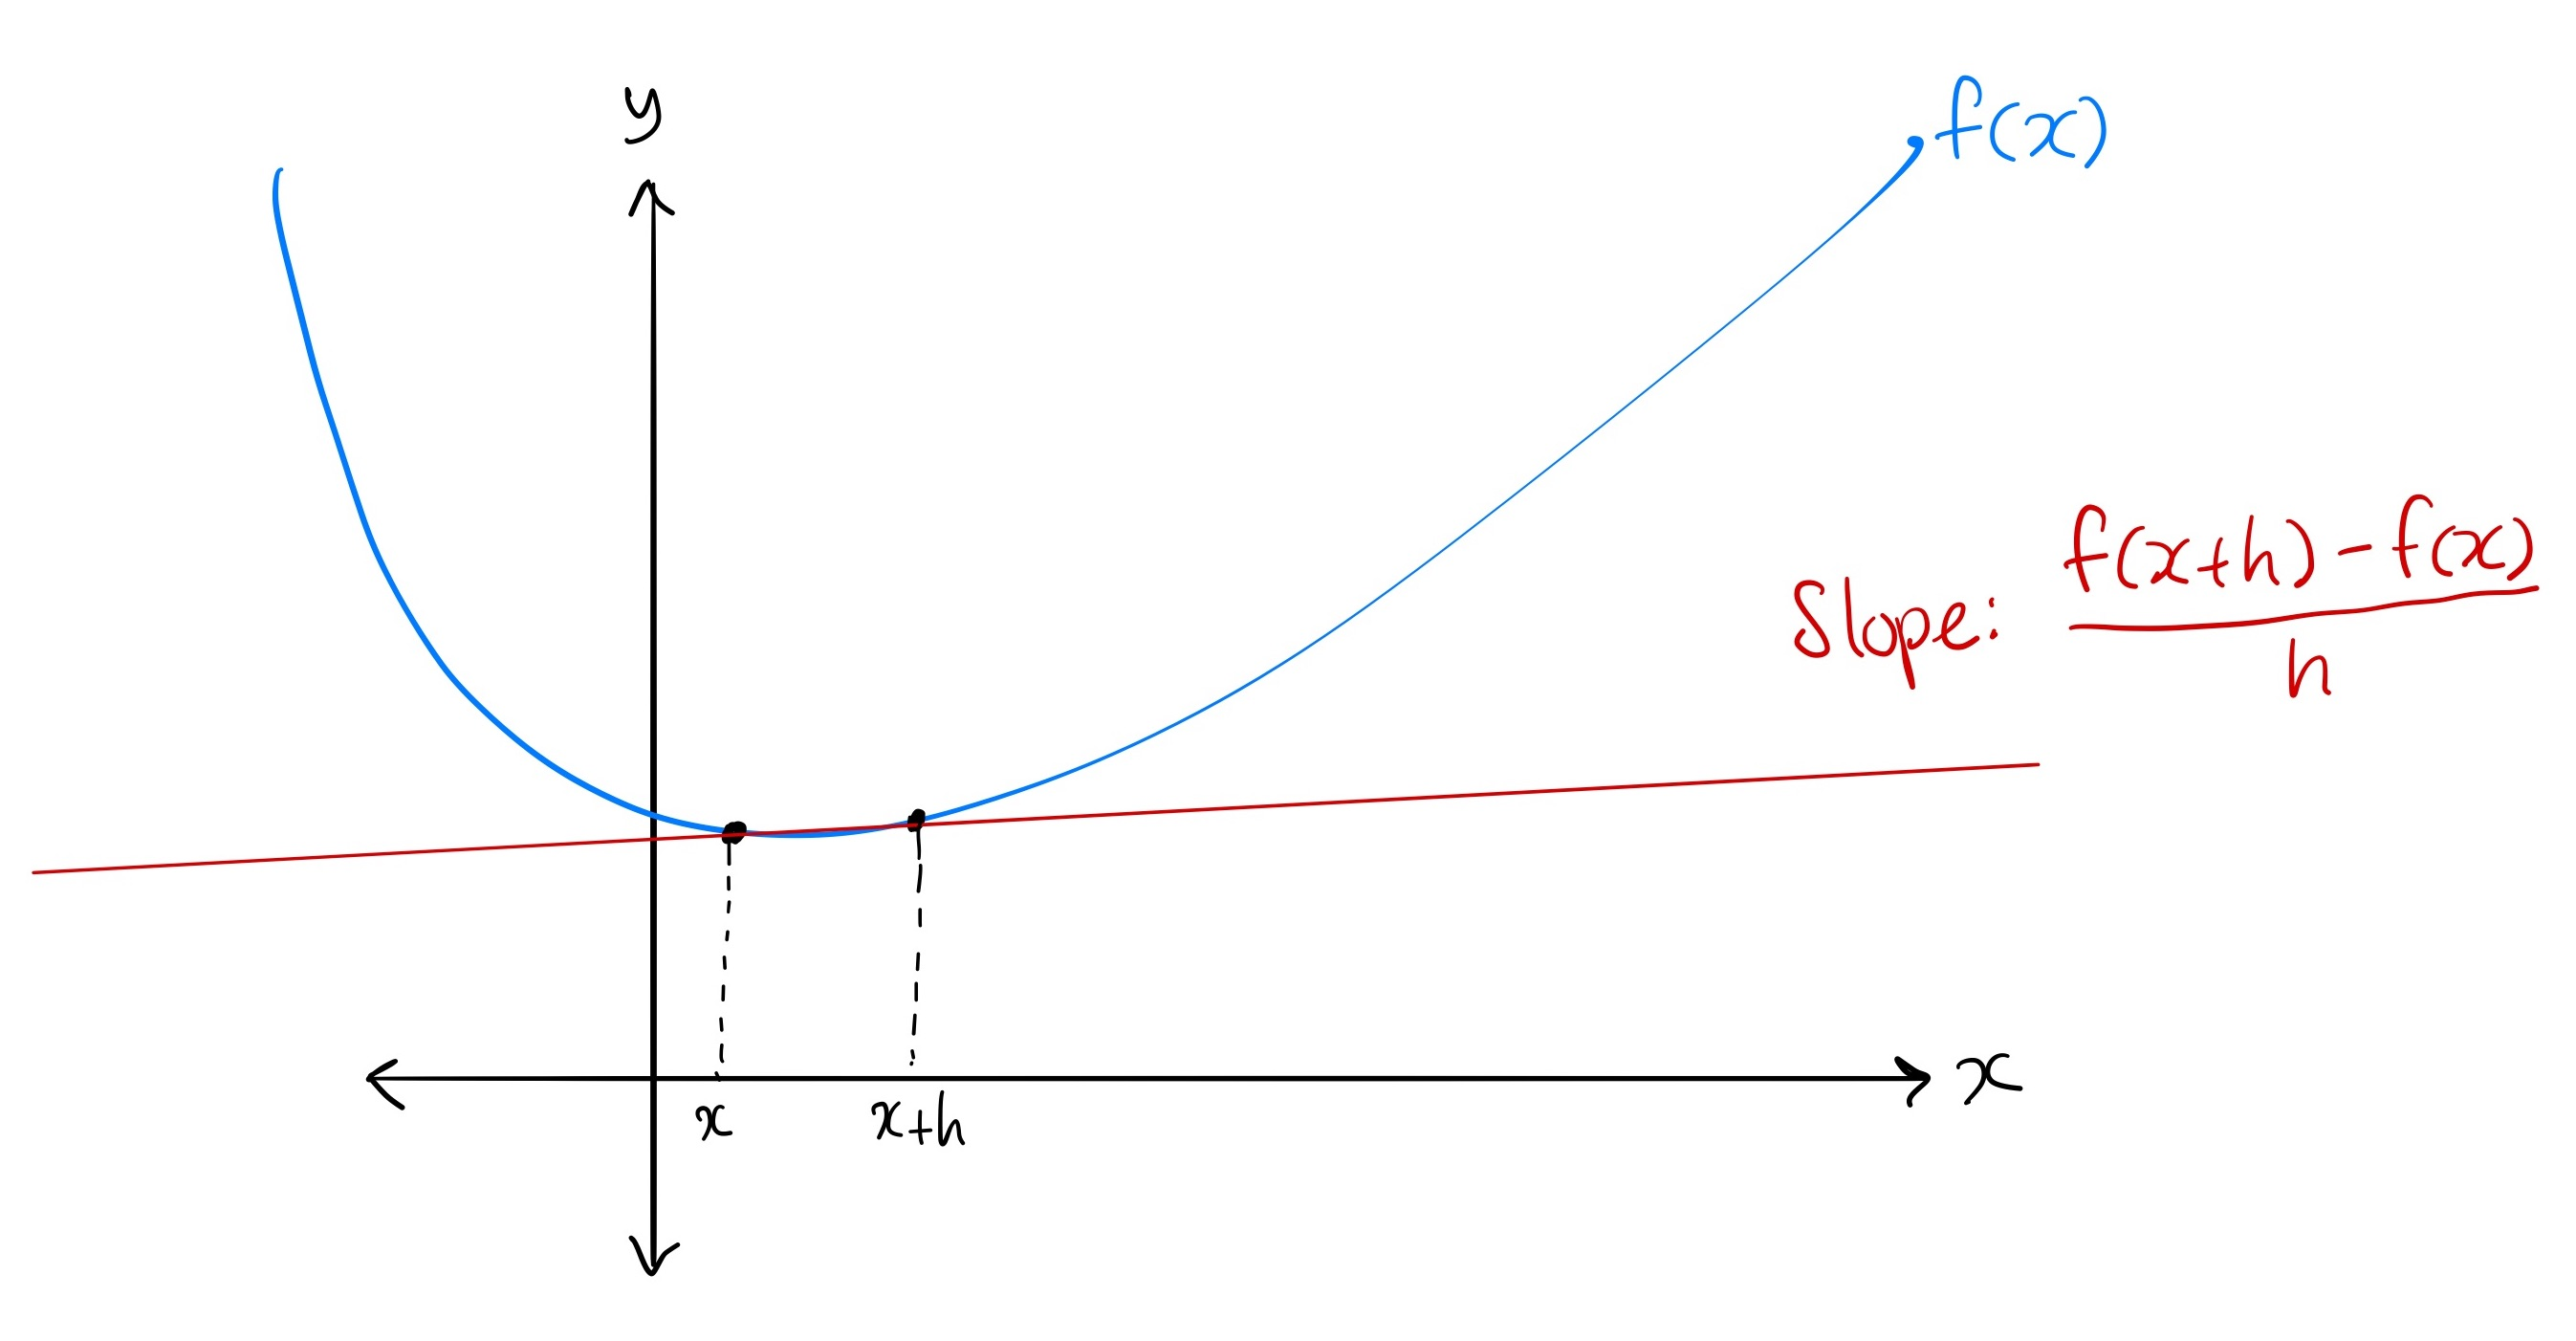
\includegraphics[width=0.7\textwidth]{derivative.jpg}
\end{center}

For the derivative to exist at a point $x$, we require
$$
\lim_{h \to 0^-} \frac{f(x + h) - f(x)}{h} = \lim_{h \to 0^+} \frac{f(x + h) - f(x)}{h}.
$$

\begin{example}
	The function $f(x) = |x|$ is not differentiable at $x = 0$, but it is everywhere else.
\end{example}

There are a number of ways of writing derivatives.
\begin{itemize}
	\item \emph{Leibniz Notation}. $\frac{df}{dx}$
	\item \emph{Lagrange Notation}. $f'(x)$
	\item \emph{Newton Notation}. $\dot{f}(x)$ -- This is typically only used for the derivative with respect to time.
\end{itemize}


For sufficiently smooth functions (the derivative exists at each step), we can define `higher order derivatives' recursively.

\begin{definition}[Higher-Order Derivatives]
	We define the notion of higher order derivatives recursively with
	$$
	\frac{d^0 f}{dx^0} = f \quad \text{and} \quad \frac{d}{dx} \left(\frac{d^n f}{dx^n}\right) = \frac{d^{n + 1} f}{dx^{n + 1}}.
	$$
	In Lagrange notation, we write $\frac{d^n f}{dx^n} = f^{(n)}(x)$.
\end{definition}

\subsection{Rules for Differentiation}

In this section, we review some rules for computing derivatives that should be familiar to you. These can be proven directly from the definitions.

\begin{theorem}[The Chain Rule]
	Consider $f(x) = F(g(x))$. Then
	$$
	f'(x) = F'(g(x)) \cdot g'(x) = \frac{dF}{dg} \cdot \frac{dg}{dx}.
	$$
\end{theorem}

\begin{theorem}[The Product Rule]
	Consider $f(x) = u(x) v(x)$. Then
	$$
	\frac{df}{dx} = u'(x) v(x) + u(x) v'(x).
	$$
\end{theorem}

We can generalise the product rule to higher order derivatives. The generalisation bears a large resemblance to the binomial theorem.

\begin{theorem}[Leibniz Rule]
	Consider $f(x) = u(x) v(x)$. Then
	$$
f^{(n)}(x) = \sum_{k = 0}^{n} \binom{n}{k} u^{(k)}(x) v^{(n - k)} (x).
	$$
\end{theorem}
\begin{proof}[Proof Sketch]
	Induction on $n$.
\end{proof}

For example, for $n = 3$ we have
$$
f'''(x) = u'''v + 3 u'' v' + 3 u' v'' + u v'''.
$$

\subsection{Order of Magnitude}

Suppose you wished to compare the `size' of two functions, in the vicinity of some specific points (that is, you want to study its behaviour locally, not globally). 
We can do this by utilizing two concepts: Little-$o$ and Big-$O$.

\begin{definition}[Little-$o$]
	We say that $f(x) = o(g(x))$ as $x \rightarrow x_0$ if
	$$
\lim_{x \to x_0} \frac{f(x)}{g(x)} = 0.
	$$
\end{definition}

Informally, we can think `$f(x)$ is much smaller than $g(x)$ around $x_0$'.

\begin{example}
	$x^2 = o(x)$ as $x \rightarrow 0$, because
	$$
	\lim_{x \to 0} \frac{x^2}{x} = 0.
	$$
\end{example}

\begin{definition}[Big-$O$]
	We say that $f(x) = O(g(x))$ as $x \rightarrow x_0$ if:
	\begin{enumerate}[label=(\roman*)]
		\item $x_0$ is finite, and $\exists m , \delta \in \R^{+}$ such that $\forall x$ where $|x - x_0| < \delta$, we have $|f(x)| \leq M | g(x)|$.
		\item $x_0$ is infinite, and $\exists$ constants $m, x_1 \in \R^{+}$ such that $\forall x > x_1$, $|f(x)| \leq M |g(x)|$.
	\end{enumerate}
\end{definition}

\begin{example}
	$x^2 = O(x)$ as $x \rightarrow 0$. To see this, take $\delta = 1$ and $M = 1$. We also have $x \neq O(x^2)$ as $x \rightarrow 0$.
\end{example}

By convention, we choose the most restrictive bound.

Consider the equation of the tangent to $f(x)$ at $x = x_0$. The slope of this tangent is given by
$$
\left.\frac{d f}{d x}\right|_{x=x_0} = \frac{f(x_0 + h) - f(x)}{h} + \frac{o(h)}{h}, \quad \text{as } h \rightarrow 0. 
$$
This implies that
$$
f(x_0 + h) = f(x_0) + f'(x_0) h + o(h), \quad \text{as } h \rightarrow 0.
$$

\subsection{Taylor Series}

Let's suppose that we wanted to approximate a well-behaved function $f(x)$ by a polynomial of degree $n$,
$$
f(x) \approx a_0 + a_1 x + \cdots + a_n x^n.
$$
Note that if we differentiate $f(x)$, we get
\begin{align*}
	f'(x) &\approx a_1 + 2a_2 x + \cdots + n a_n x^{n - 1} \\
	\text{and} \quad f''(x) &\approx 2a_2 + \cdots + (n- 1)n a_n x^{n - 2} \\
	&\vdots
\end{align*}
If we evaluate all of these at $x = 0$, we get
$$
f(0) \approx a_0, f'(0) \approx a_1, f''(0) \approx 2a_2, \cdots, f^{(n)}(0) \approx n! a_n.
$$
Thus, given that we are trying to approximate $f(x)$ with our polynomial, it would make sense teo try and match these coefficients with the derivatives of $f(x)$. This gives us the series
$$
p_n(x) = f(0) + x f'(0) + \cdots + \frac{x^n}{n!} f^{(n)}(0).
$$

Now we considered this about the point $0$, but we could have just as easily chosen any other point $x_0$ to approximate the function at. This gives us the concepts of a taylor polynomial.

\begin{definition}
For a sufficiently well-behaved function $f(x)$, we define the \vocab{taylor polynomial of degree $n$} to be
$$
p_n(x) = f(x_0) + (x - x_0) f'(x_0) + \cdots + \frac{(x - x_0)^n}{n!} f^{(n)}(x_0).
$$
\end{definition}

Recall from the ast lecture that
$$
f(x + h) = f(x) + hf'(x) + o(h), 
$$
as $h \rightarrow 0$. This can be generalized, provided the first $n$ derivatives of $f$ all exist.
\begin{theorem}
	For a well behaved function $f(x)$, we have
	$$
	f(x + h) = f(x) + h f'(x) + \frac{h^2}{2} f''(x) + \cdots + \frac{h^n}{n!} f^{(n)}(x) + o(h^n).
	$$
\end{theorem}
\begin{proof}[Proof Sketch]
	Integrate and then induct.
\end{proof}

Indeed, this is reminiscent of the taylor polynomial and indeed we can use it to say something about the size of the error. 



% Informal treatment of differentiation as a limit, the chain rule, Leibnitz's rule, Taylor series, informal treatment of $O$ and $o$ notation and l'Hôpital's rule; integration as an area, fundamental theorem of calculus, integration by substitution and parts.

% Informal treatment of partial derivatives, geometrical interpretation, statement (only) of symmetry of mixed partial derivatives, chain rule, implicit differentiation. Informal treatment of differentials, including exact differentials. Differentiation of an integral with respect to a parameter.

% \section{First-Order Linear Differential Equations}

% Equations with constant coefficients: exponential growth, comparison with discrete equations, series solution; modelling examples including radioactive decay.

% Equations with non-constant coefficients: solution by integrating factor.

% \section{Nonlinear First-Order Equations}

% Nonlinear first-order equations Separable equations. Exact equations. Sketching solution trajectories. Equilibrium solutions, stability by perturbation; examples, including logistic equation and chemical kinetics. Discrete equations: equilibrium solutions, stability; examples including the logistic map.

% \section{Higher-Order Linear Differential Equations}

% Complementary function and particular integral, linear independence, Wronskian (for second-order equations), Abel's theorem. Equations with constant coefficients and examples including radioactive sequences, comparison in simple cases with difference equations, reduction of order, resonance, transients, damping. Homogeneous equations. Response to step and impulse function inputs; introduction to the notions of the Heaviside step-function and the Dirac delta-function. Series solutions including statement only of the need for the logarithmic solution.

% \section{Multivariate Functions: Applications}

% Directional derivatives and the gradient vector. Statement of Taylor series for functions on $\mathbb{R}^{n}$. Local extrema of real functions, classification using the Hessian matrix. Coupled first order systems: equivalence to single higher order equations; solution by matrix methods. Non-degenerate phase portraits local to equilibrium points; stability.

% Simple examples of first- and second-order partial differential equations, solution of the wave equation in the form $f(x+c t)+g(x-c t)$.


Lol this is non-sense -- come back later lol.

\end{document}
